\documentclass[a4paper,10pt]{article}
\usepackage[utf8]{inputenc}
\usepackage{amsmath}
\usepackage{amsfonts}
\usepackage{amssymb}
\usepackage[german]{babel}
\setlength{\parindent}{0cm}
\usepackage{setspace}
\usepackage{mathpazo}
\usepackage{listings}
\usepackage{graphicx}
\usepackage{wasysym} 
\usepackage{booktabs}
\usepackage{verbatim}
\usepackage{ulem}
\usepackage{enumerate}
\usepackage{hyperref}
\usepackage{ulem}
\usepackage{stmaryrd }
\usepackage[a4paper,
left=1.8cm, right=1.8cm,
top=2.0cm, bottom=2.0cm]{geometry}
\usepackage{tabularx}
\usepackage{tikz}
\usetikzlibrary{trees,petri,decorations,arrows,automata,shapes,shadows,positioning,plotmarks}


\newcommand{\rf}{\right\rfloor}
\newcommand{\lf}{\left\lfloor}
\newcommand{\tabspace}{15cm}
\newcommand{\N}{\mathbb{N}}
\newcommand{\Z}{\mathbb{Z}}

\begin{document}
\begin{center}
\Large{Cognivite Algorithms: Assignment 3} \\
\end{center}
\begin{tabbing}
Tom Nick \hspace{2cm}\= - 340528\\
Maximilian Bachl \> - 341455 \\
\end{tabbing}

\section*{Exercise 2}
\begin{enumerate}
    \item The Perceptron produces highly varying results, it even outperforms the LDA at sometimes while at other times it is beaten by the NCC. 
    \item Yes, the data is optimal because the LDA makes the assumption of Gaussian distributed data. This is exactly the case with the SciPy method \texttt{multivariate\_normal}.
    \item In the used covariance matrix used for the test the upper left value of the matrix is 5 and the lower right is $0.5$. Thus the data is always stretched more from left to right than from top to bottom like it is seen in resulting plots. The NCC achieves comparable values to the LDA if the covariance matrix has equal values on the diagonal.
\end{enumerate}
\section*{Exercise 3}
It takes a set of training data and the associated labeling. Then we separate the data in two pieces: Training data $\frac 1 f$ and test data $\frac {f-1} {f}$. The algorithm is trained with the smaller part of the data and then its output vectors are used for the classification of the test part. This is done $f$ times and the accuracy values are saved and output.

The performance for the test is better. Although there is a correlation between training and test performance: An algorithm that sucks in the training won't achieve good results in the test phase.
\section*{4}
I'ld prefer the Perceptron for the digits. The digit data is not normally-distributed and thus the LDA performs very bad. 
For the normally distributed BCI data the LDA is best.\\

USPS:

\leavevmode\vadjust{\vspace{-\baselineskip}}\newline
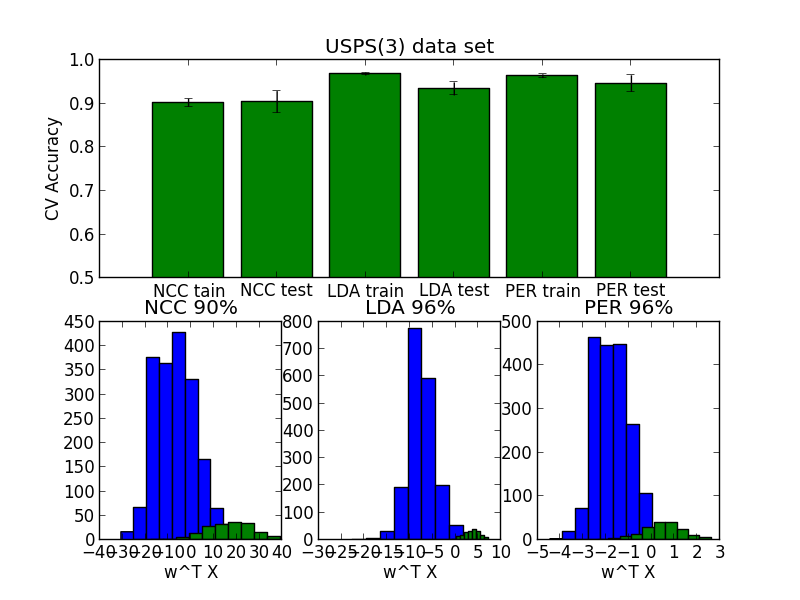
\includegraphics[scale=0.5]{usps}

BCI:

\leavevmode\vadjust{\vspace{-\baselineskip}}\newline
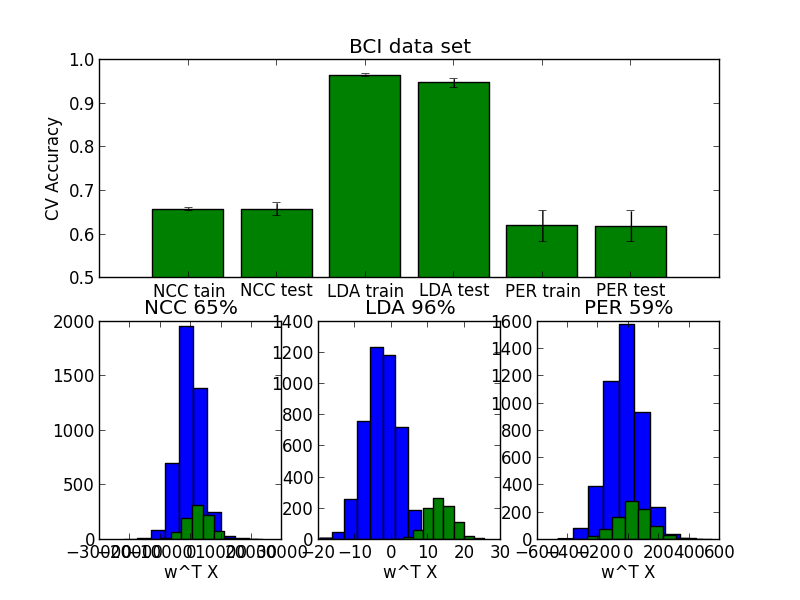
\includegraphics[scale=0.5]{bci}

\end{document}
